After removing basic English stopwords and non-alphabetic tokens, the bar chart confirmed the dominance of words like number, url, mail, date, list, get.
Their persistence highlights their potential importance or noise factor.

\begin{figure}[H]
    \centering
    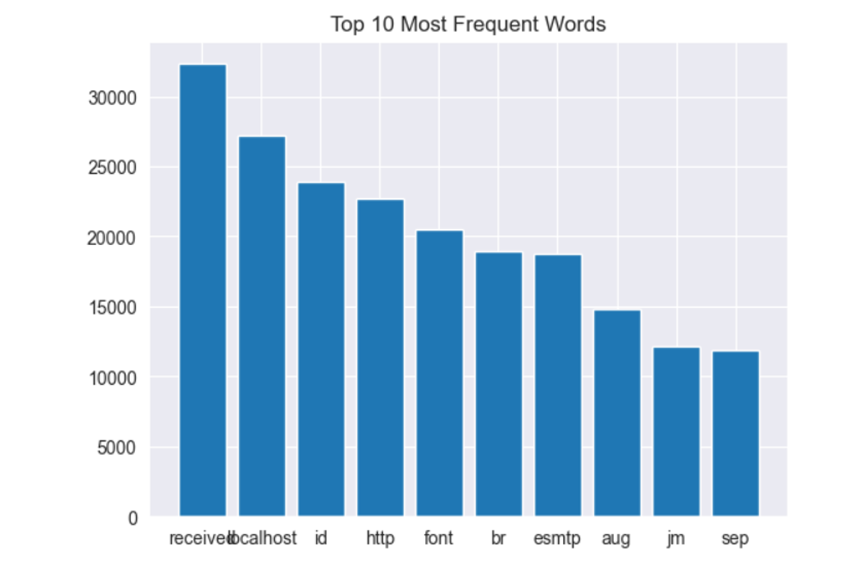
\includegraphics[width=\linewidth]{images/frequent_words}
    \caption{Bar Chart for 10 Most Frequent Words}
    \label{fig:frequent_words}
\end{figure}

The most frequent word is ``received'', with a significantly higher count (over 30,000) compared to the other top words.
This suggests that the word ``received'' appears very often in the analyzed text data after the filtering.

The following most frequent words, in descending order, are ``localhost'', ``id'', ``http'', ``font'', ``br'', ``esmtp'', ``aug'', ``jm'', and ``sep''.
These words have frequencies ranging from approximately 11,000 to 27,000.

The nature of the top words suggests the analyzed text data might be related to email headers or technical logs.
Words like ``received'', ``localhost'', ``id'', ``http'', and ``esmtp'' are commonly found in email metadata.
``aug'' and ``sep'' likely refer to month abbreviations.
``font'' and ``br'' could appear in the content or formatting information.

The code successfully identifies and counts the occurrences of words after applying basic text cleaning.
The use of nltk.word\_tokenize splits the text into individual words, .lower() converts them to lowercase for consistent counting, and the list comprehension filters out non-alphabetic tokens and common English stop words.

The Counter object efficiently calculates word frequencies, and most\_common(10) retrieves the top 10 most frequent words and their counts.
This data is then used to generate the bar chart using matplotlib.pyplot.

The visualization clearly shows the relative frequency of the top 10 words.
The height of each bar directly corresponds to the number of times that word appears in the processed text.
